\chapter{SONUÇLAR}

Bu tez çalışması sonucunda güç, endüstri ve kullanıcı elektroniğinde kullanılan ARM tabanlı denetleyicilerin, programlamlaması ve Nesnelerin İnternetin ile ortaya çıkan ihtiyaçlara bir çözüm sunulmuştur. Kullanıcı platfordan bağımsız olarak cihaza bağlanıp, hedef cihazın yazılım güncellenmsi, hedef cihazın istenilen hafıza adresindeki verinin belirlenen aralıklarda gerçek zamanlı olarak ölçülmesi, RS232 portu ile hedef cihazdan okunan veriler cihazda zaman domeninde kaydedilip, istenildiği zaman bu veriler ile grafik çizimi ve verilerin \acrfull{CSV} formatında kullanıcı cihazına kaydedebilmektedir. Sistem tasarımı Şekil \ref{fig:sistem}'de gösterilmiştir.

\begin{figure}[h]
\centering
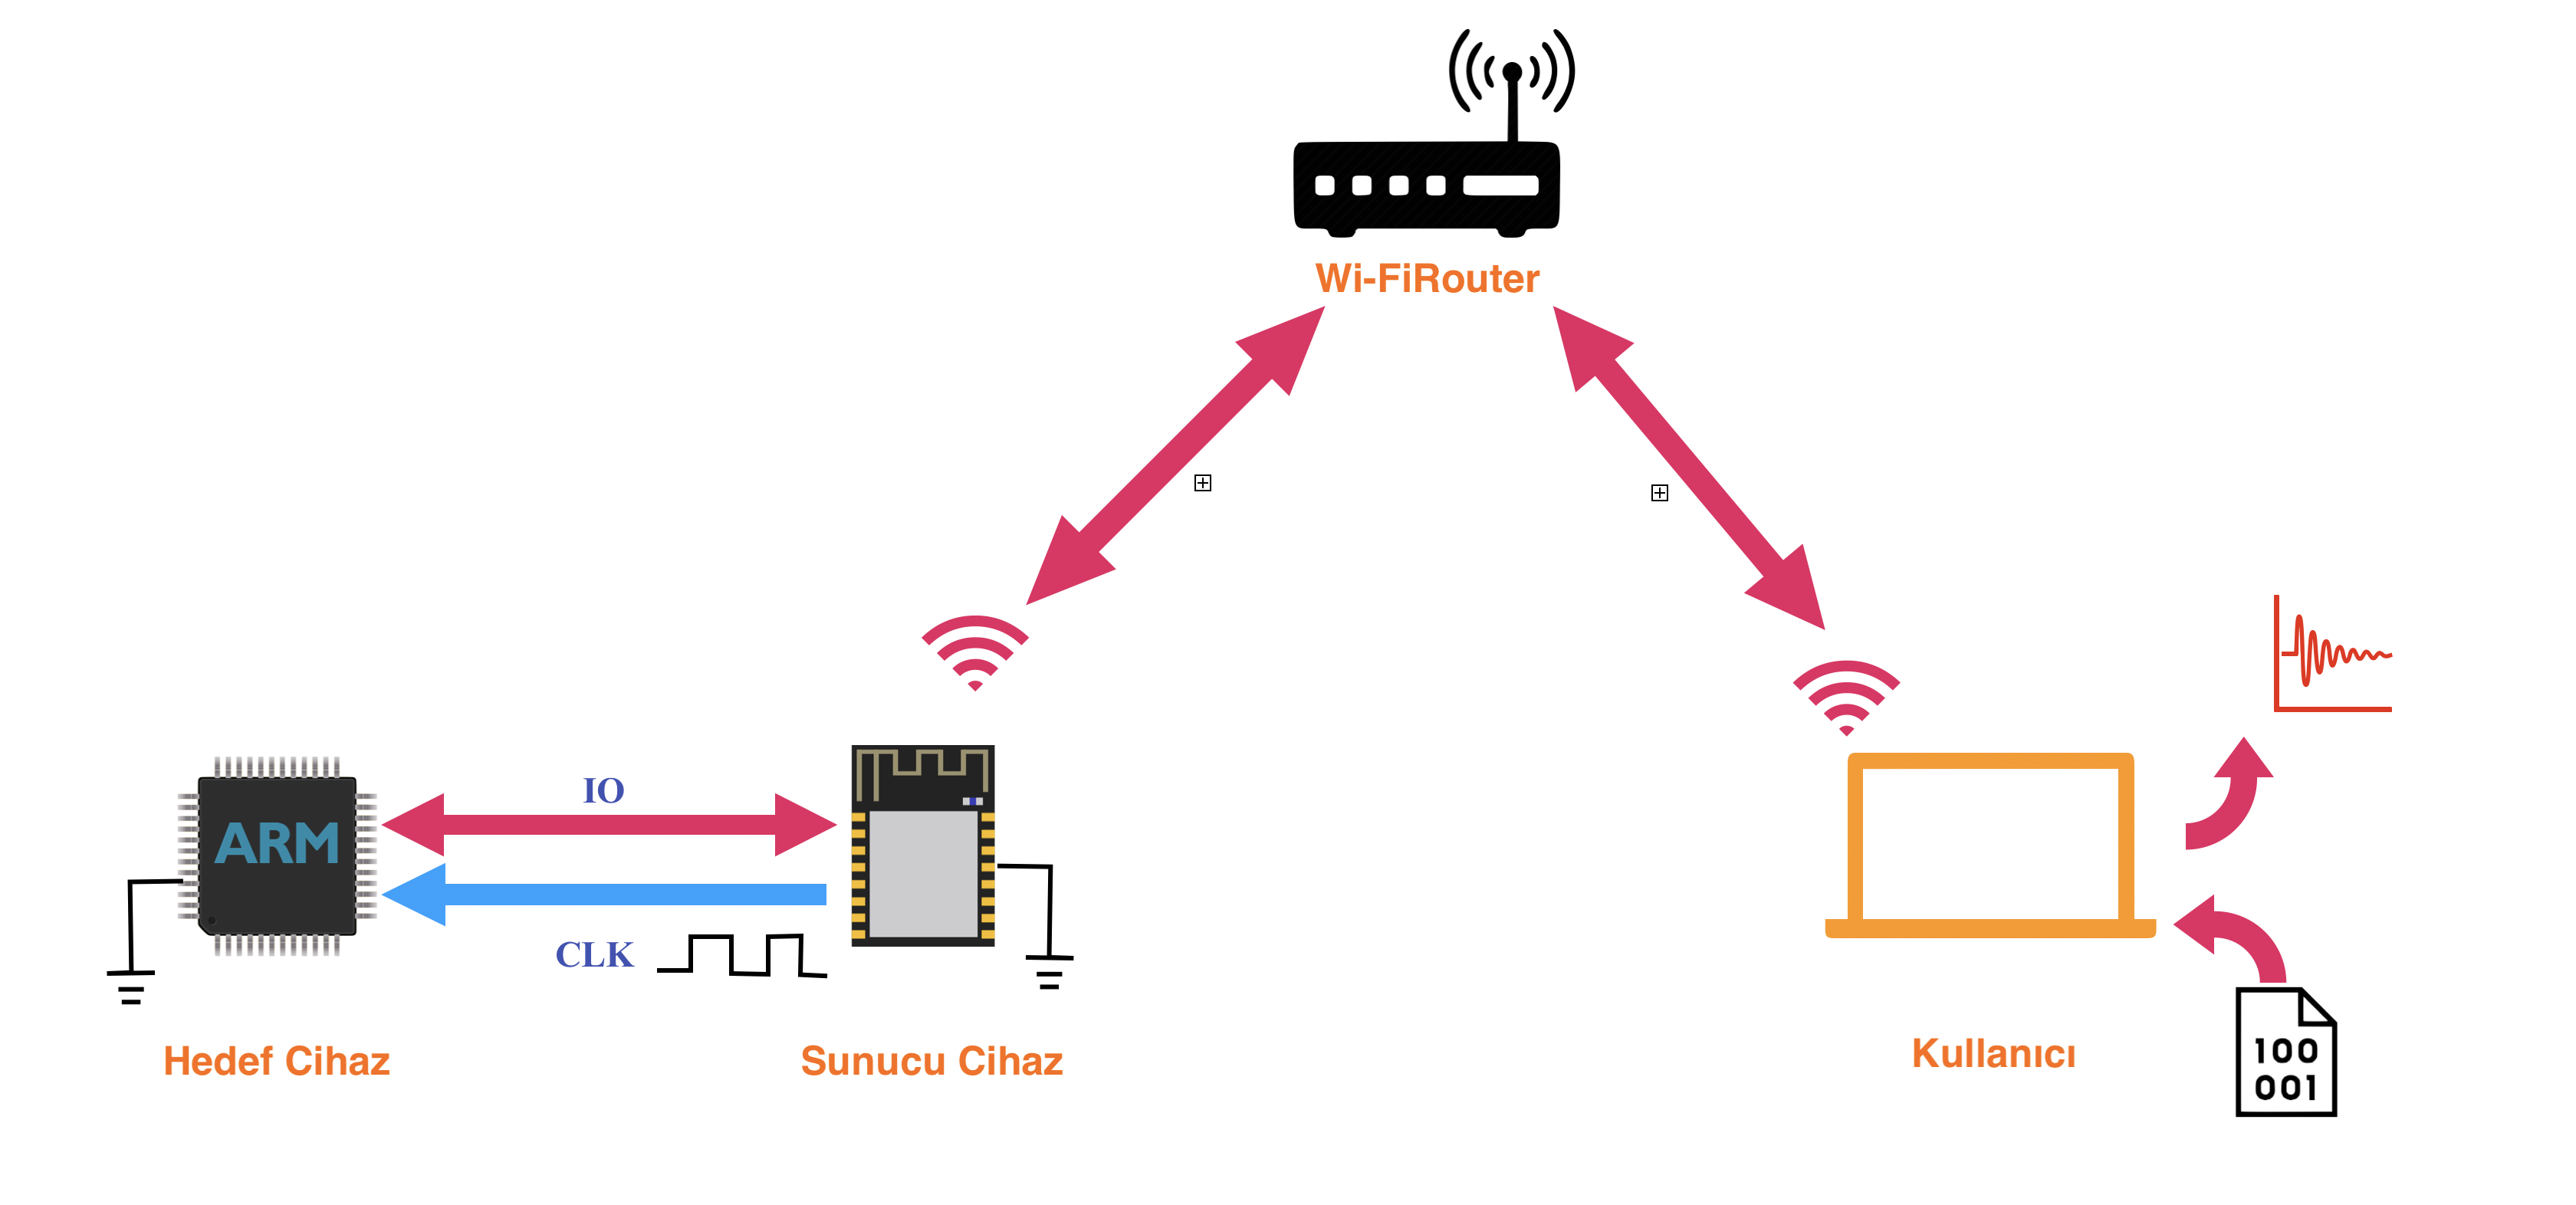
\includegraphics[width=\textwidth]{gorseller/sistem}
\caption{Sistem Tasarımı}\label{fig:sistem}
\end{figure}

Çalışma sonucunda ortaya çıkan ürün ile hedef cihaz, yerel ağ üzerinde veri aktarımı ve programlanması sağlanmıştır. Ancak sunucu cihazın bulunduğu ağda, cihaz için port açıldığında ya da sunucu cihaz ile kullanıcı arasındaki iletişim başka bir sunucu tarafından sağlandığında kullanıcı konumdan bağımsız olarak internet erişimi olan herhangi bir ağ üzerinden hedeflenen amaçların tümünü gerçekleştirebilir.

\begin{figure}[h]
\centering
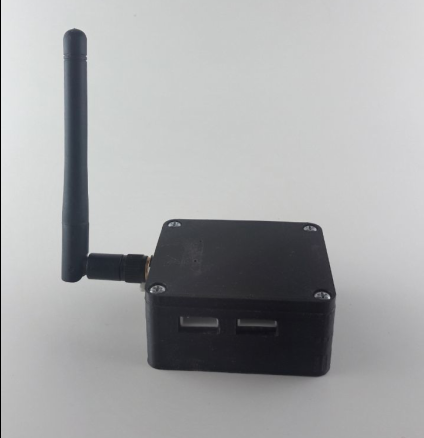
\includegraphics[width=0.7\textwidth]{gorseller/product}
\caption{Çalışma Sonucunda Elde Edilen Ürün}\label{fig:product}
\end{figure}

